 
\documentclass{beamer}

\usepackage{tikz}
\usetikzlibrary{arrows}

\usepackage{amsmath}

\title{Brain mapping tools for neuroscience research}
\author{Devin Crowley (\texttt{devin.g.crowley@gmail.com})}
\date{}

\institute{NeuroData and Center for Imaging Science\\
Department of Biomedical Engineering\\
Johns Hopkins University}


\usetheme{default}
%\renewcommand{\insertnavigation}[1]{}
\setbeamertemplate{headline}{}
\setbeamertemplate{footline}[text line]{%
  \parbox{\linewidth}{Devin Crowley (\texttt{devin.g.crowley@gmail.com}) \hfill Johns Hopkins University \hfill Brain mapping tools for neuroscience}}
  
\beamertemplatenavigationsymbolsempty
\renewcommand{\footnotesize}{\tiny}

% footnote with no number
\newcommand\blfootnote[1]{%
  \begingroup
  \renewcommand\thefootnote{}\footnote{#1}%
  \addtocounter{footnote}{-1}%
  \endgroup
}

\begin{document}
\begin{frame}
\maketitle
\end{frame}



%\begin{frame}{What is brain mapping?}
%
%Assigning a standard coordinate to each point in a neuroimage.
%
%I think this is a very weak first slide
%
%\end{frame}


\begin{frame}{Workshop Outline}

\begin{enumerate}
\item Focused look at registration algorithms
\item Running code on real data
\item Discussion of issues affecting the community
\end{enumerate}

\end{frame}

\begin{frame}{The goal of brain mapping}

%Registration: , Annotation: , Morphometry: 


% my picture will have an target (top left), a atlas (top right), and a deformation (bottom center)

\begin{tikzpicture}
\tikzstyle{rect} = [rectangle, thick, minimum width=2cm, minimum height=2cm, text centered, text width=3.5cm, draw=black, fill=black!10];
\tikzstyle{arrow} = [->, thick, line width=1mm];

\node (target) [rect ] at (-3.5,0) {Experimental data 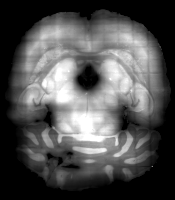
\includegraphics[width=\textwidth]{ex1_target_slice.png}};
\node (atlas) [rect]  at (3.5,0) {Standard coordinates 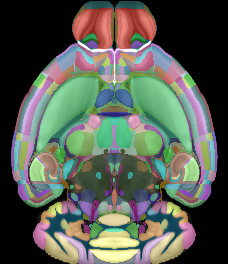
\includegraphics[width=\textwidth]{ex1_allen_slice.png}};
\node (map) [rectangle, text width=3cm, text centered, ] at (0,-0) {3. Transformation 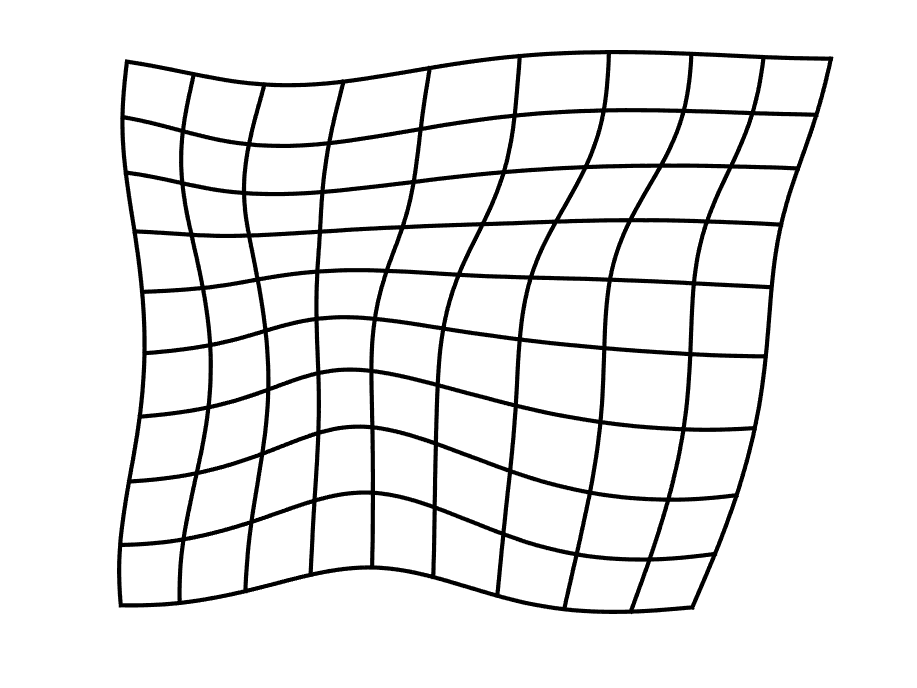
\includegraphics[width=2.75cm,clip,trim=0.5in 0in 0.5in 0in]{ex1_warp.png}};

\draw [arrow] (target) to [out=45,in=135] node [anchor=south] {1. Registration} (atlas);
\draw [arrow] (atlas) to [out=-135,in=-45] node [anchor=north] {2. Interpretation} (target);

\end{tikzpicture}
\end{frame}

\begin{frame}{1. Registration}



Align images into a standard coordinate system

\begin{tikzpicture}
\tikzstyle{rect} = [rectangle, thick, text centered, text width=1.4cm, fill=black!10];
\tikzstyle{arrow} = [->, thick, line width=0.5mm];


\node (mni) [rect] at (0,0) {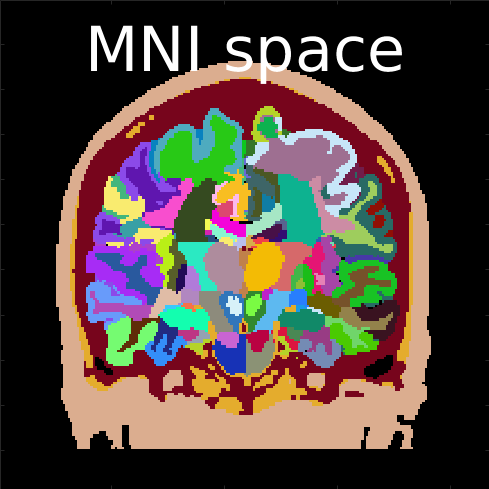
\includegraphics[width=\textwidth]{reg_mni}};



\node (im1a) [rect] at (-4.5,1) {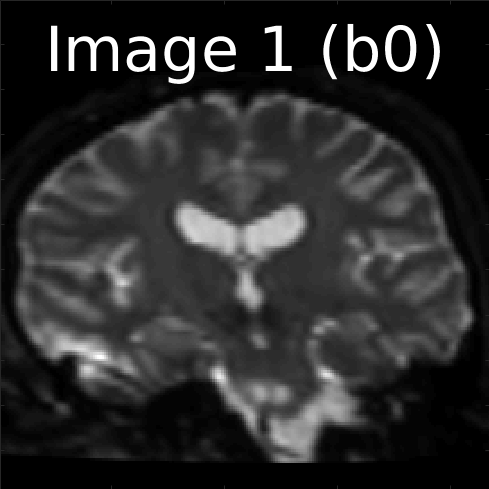
\includegraphics[width=\textwidth]{reg_1a}};



\node (im2a) [rect] at (4.5,1) {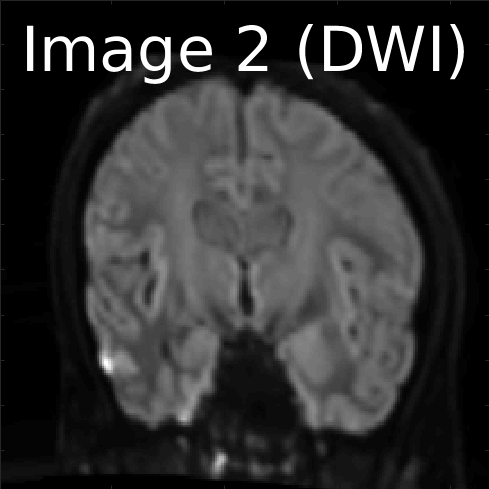
\includegraphics[width=\textwidth]{reg_2a}};



\node (im4a) [rect] at (4.5,-1) {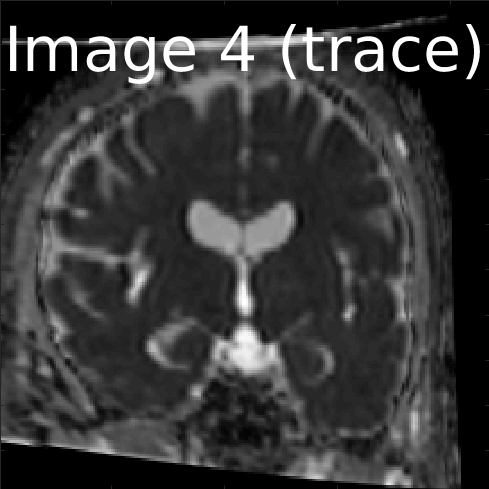
\includegraphics[width=\textwidth]{reg_4a}};


\node (im3a) [rect] at (-4.5,-1) {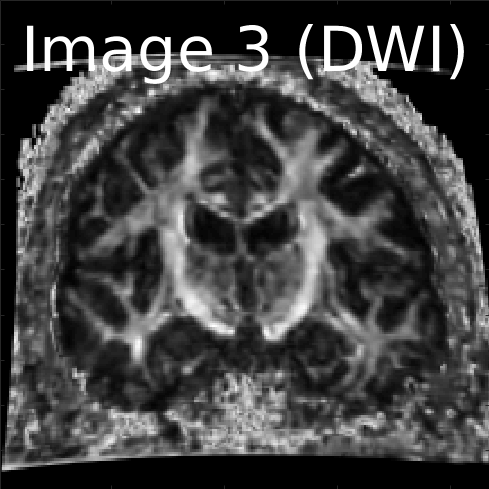
\includegraphics[width=\textwidth]{reg_3a}};

\draw [arrow](im1a) -- (mni);
\draw [arrow](im2a) -- (mni);
\draw [arrow](im3a) -- (mni);
\draw [arrow](im4a) -- (mni);


\uncover<2->{
\node (im2b) [rect] at (-2,0.9) {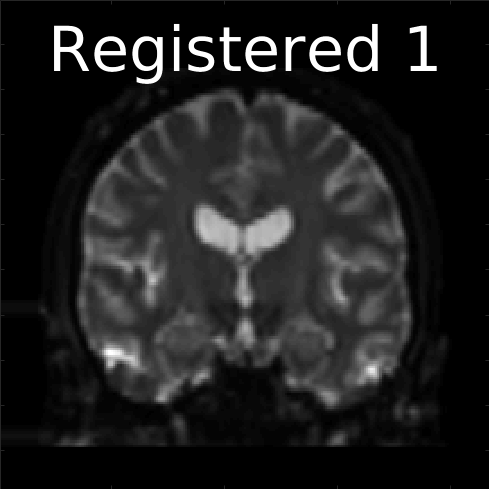
\includegraphics[width=\textwidth]{reg_1b}};
\node (im2b) [rect] at (2,0.9) {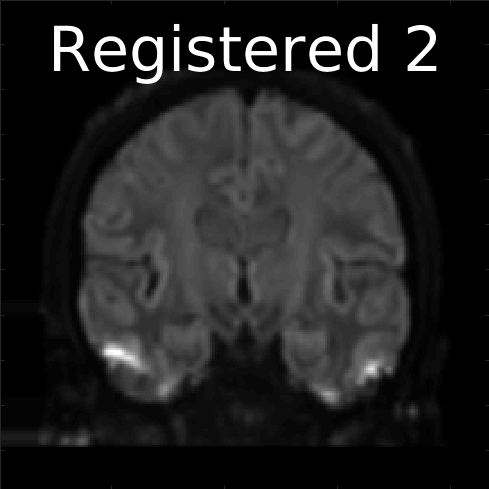
\includegraphics[width=\textwidth]{reg_2b}};
\node (im2b) [rect] at (2,-0.9) {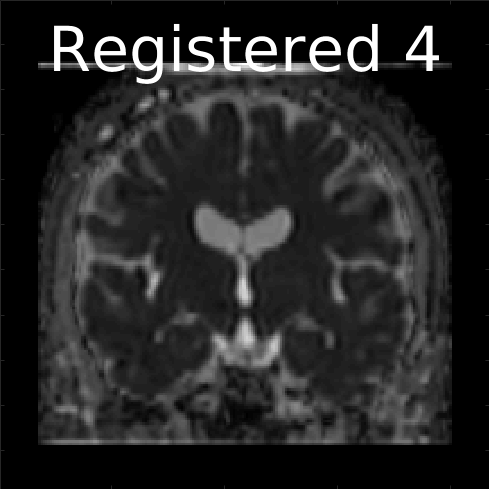
\includegraphics[width=\textwidth]{reg_4b}};
\node (im2b) [rect] at (-2,-0.9) {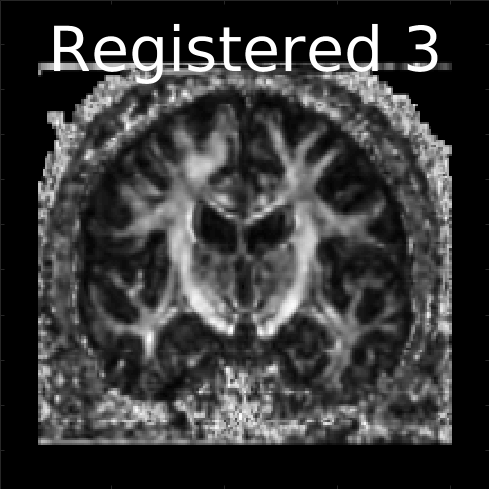
\includegraphics[width=\textwidth]{reg_3b}};
}
\end{tikzpicture}



\begin{itemize}
\item 
Enrich information by fusing modalities


\item
Analyze different specimens statistically

\item 
Build databases of information indexed to spatial coordinates

\end{itemize}

\end{frame}



\begin{frame}{2. Interpretation}


Leverage information stored in atlas coordinates.\footnote{MBA: Mouse brain architecture \url{brainarchitecture.org}, ARA: Allen reference atlas \url{connectivity.brain-map.org/}}

\begin{minipage}{0.3\textwidth}
MBA
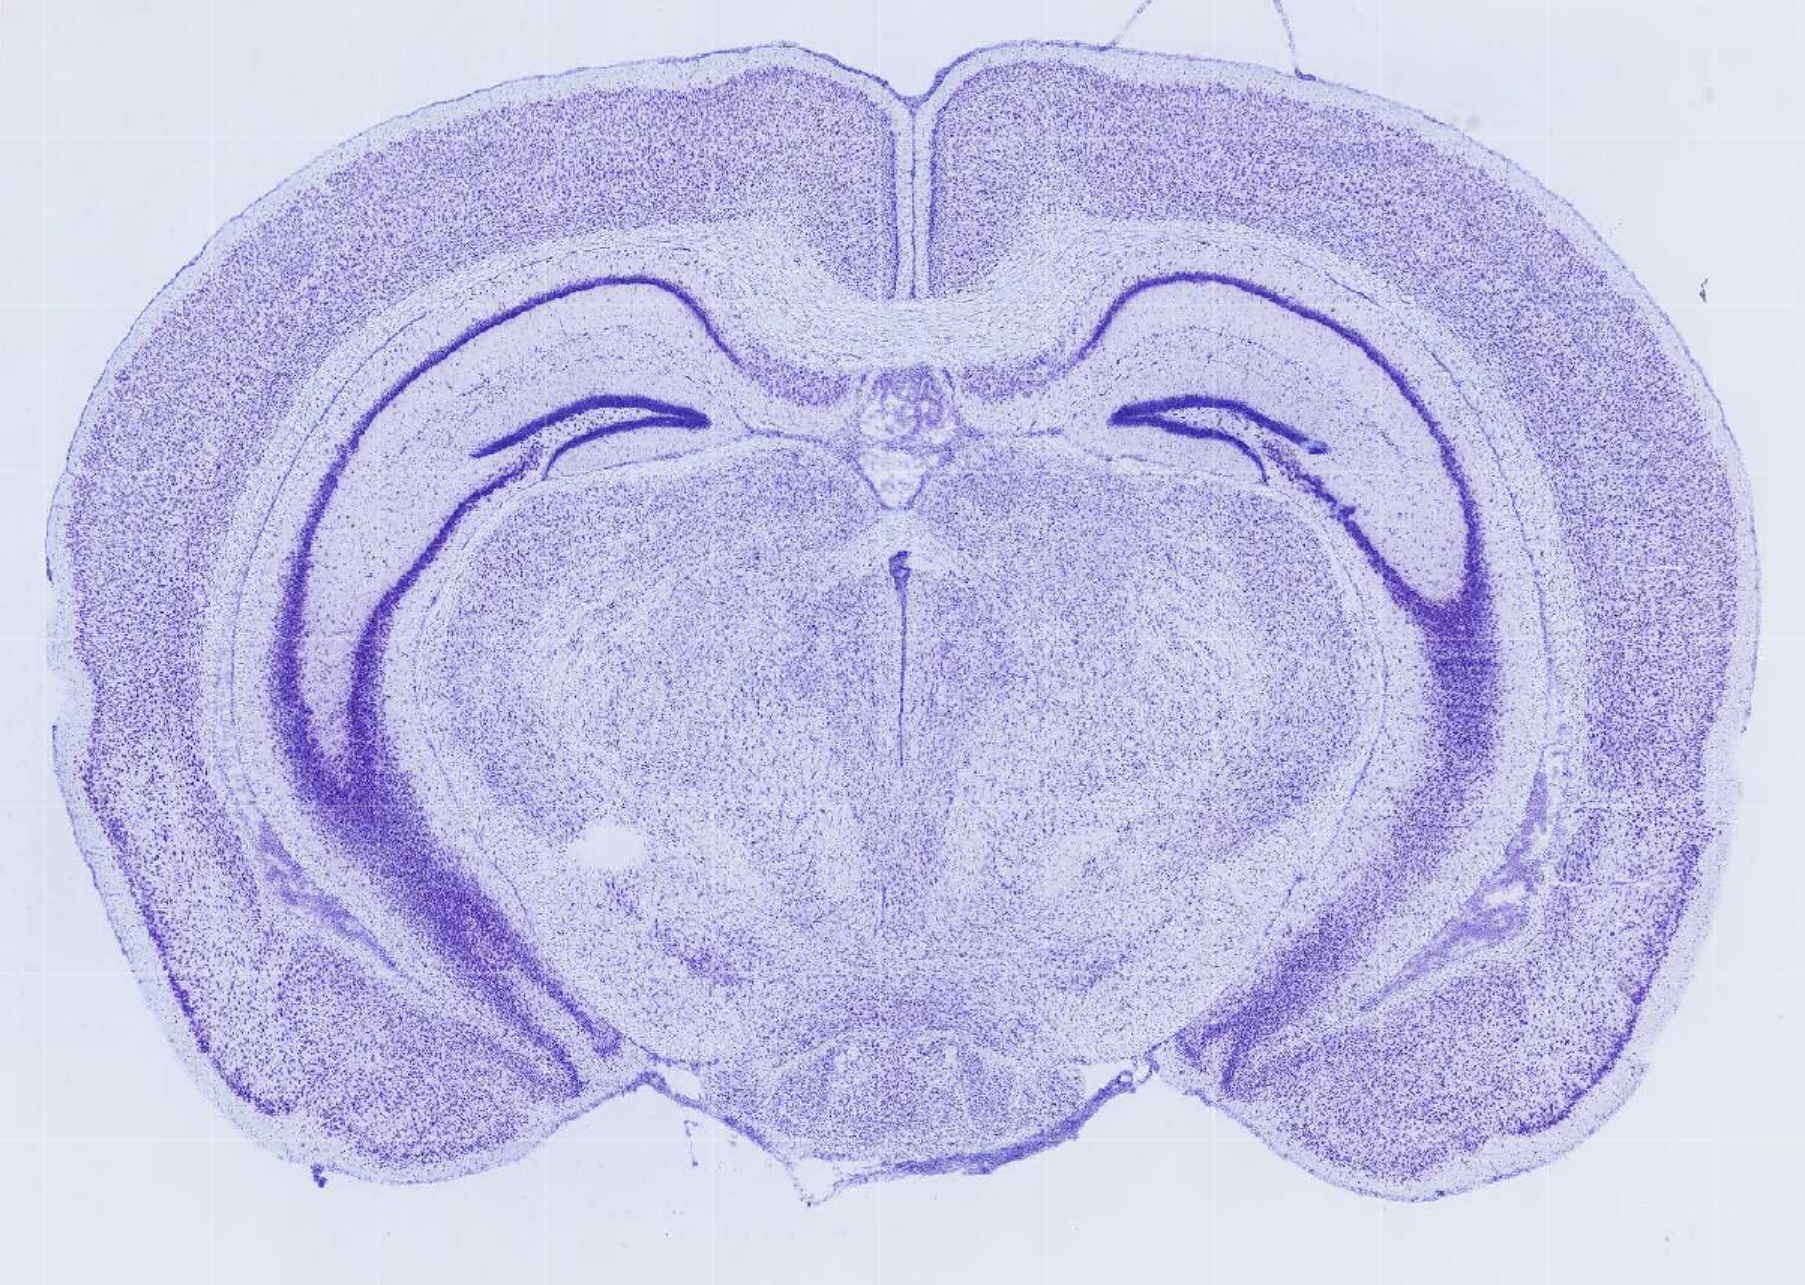
\includegraphics[width=\textwidth]{mba2.png}\\
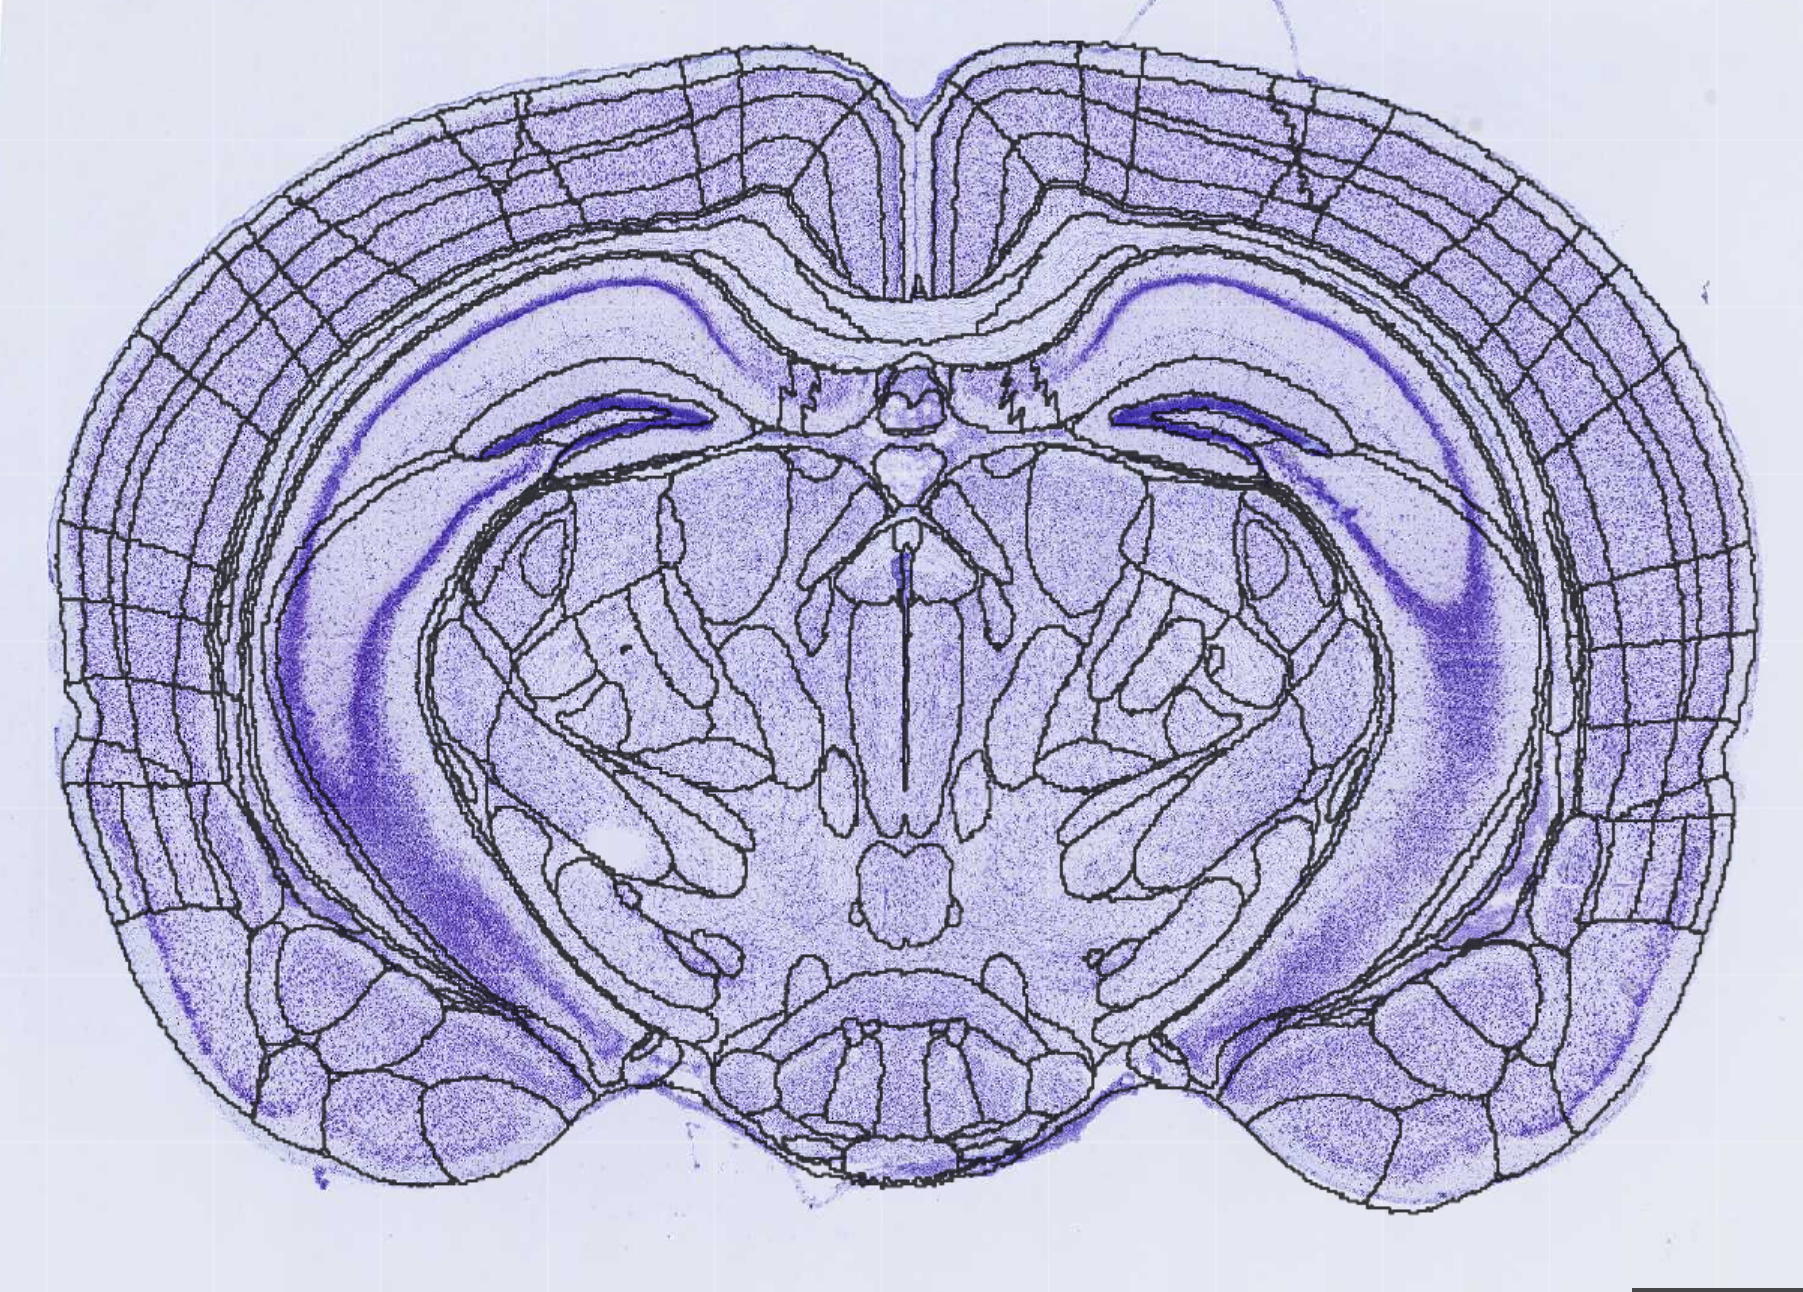
\includegraphics[width=\textwidth]{mba1.png}
\end{minipage}~
\begin{minipage}{0.7\textwidth}
ARA\\
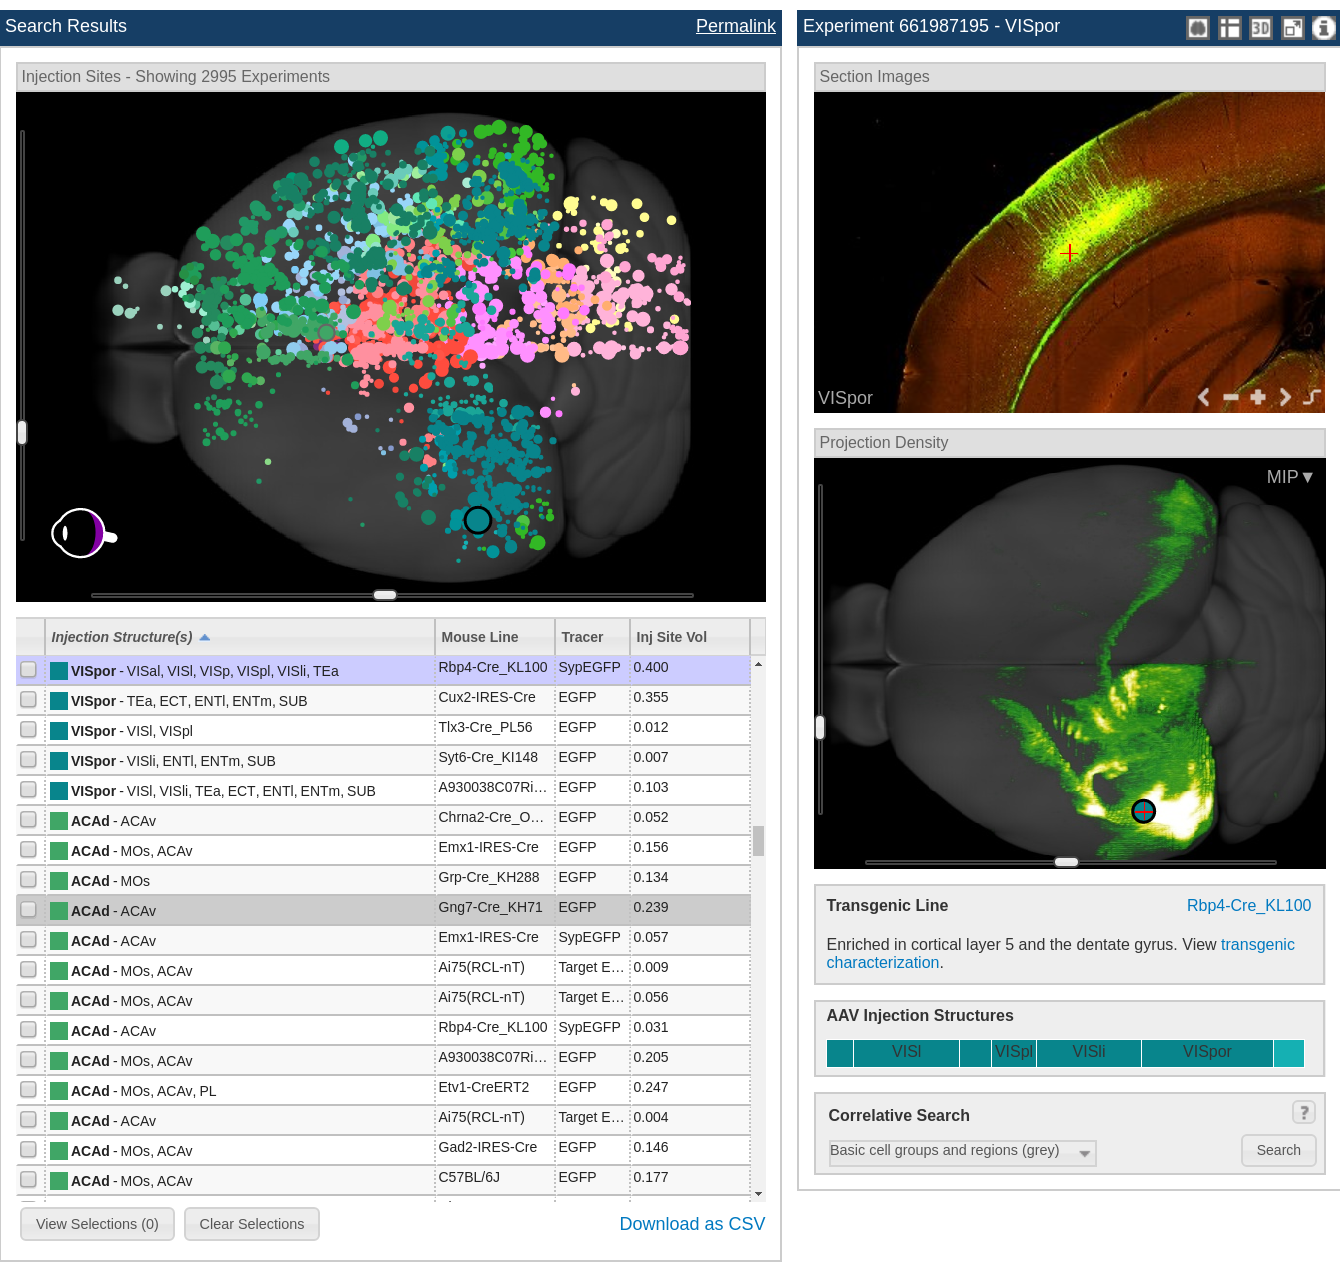
\includegraphics[width=\textwidth,clip,trim=1in 6in 1in 1.5in]{allen-connectivity}
\end{minipage}

\begin{itemize}

\item
Label images with standard ontologies

\item
Index to gene expression, cell types, tractography, etc.

\end{itemize}
\end{frame}


\begin{frame}{3. Transformation}

Studying transformations quantifies growth or atrophy %(morphometry).
\vspace{-0.5em}
\begin{center}
\only<1>{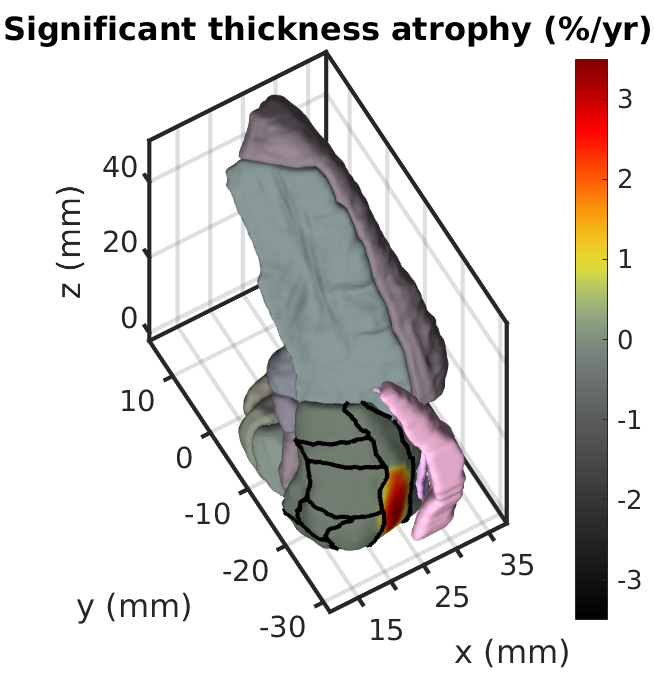
\includegraphics[width=0.45\textwidth]{v10kavli_daniel_thickness_sig.png}}%
\only<2>{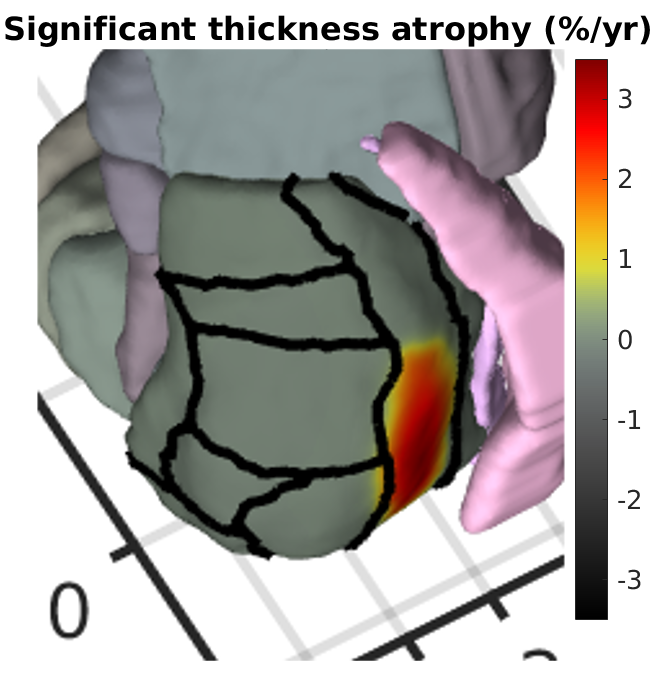
\includegraphics[width=0.45\textwidth]{v10kavli_daniel_thickness_sig-edit.png}}%
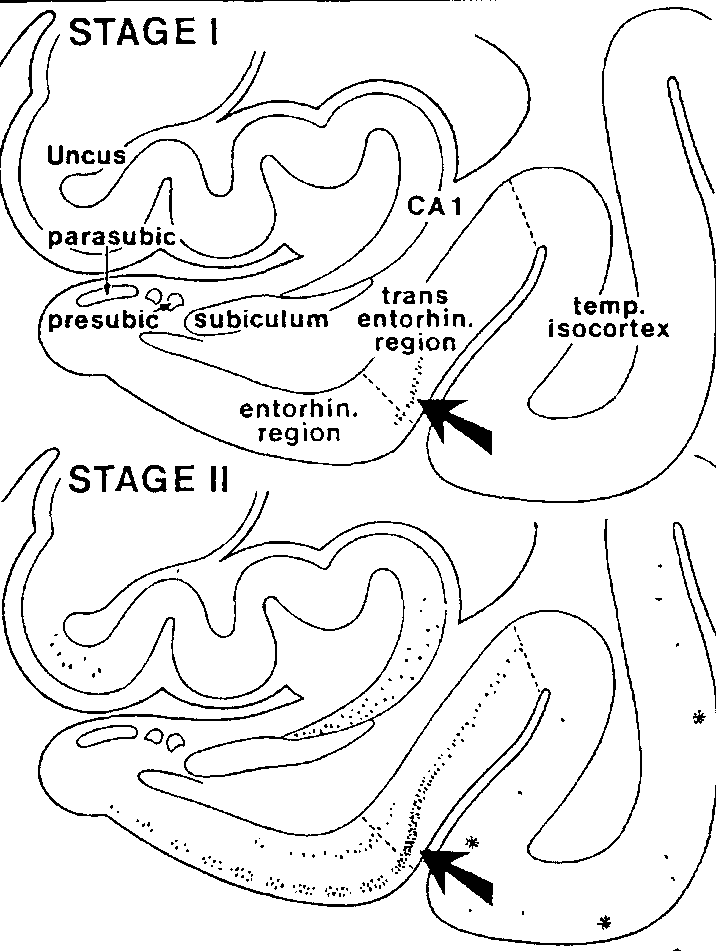
\includegraphics[width=0.3\textwidth]{braak12.png}
\end{center}
\vspace{-1em}
\begin{itemize}
\item Here thickness change in transentorhinal region measured from longitudinal MRI\footnote{Tward, Daniel J., et al. ``Entorhinal and transentorhinal atrophy in mild cognitive impairment using longitudinal diffeomorphometry.'' Alzheimer's \& Dementia: Diagnosis, Assessment \& Disease Monitoring 9 (2017): 41-50.}
\item Previously only observed at autopsy
\end{itemize}

\end{frame}










\begin{frame}{The ingredients of a brain mapping tool}

Mappings are calculated from optimization problem with 3 parts.

\vspace{1em}

Transformation model: What types of mappings do we consider?

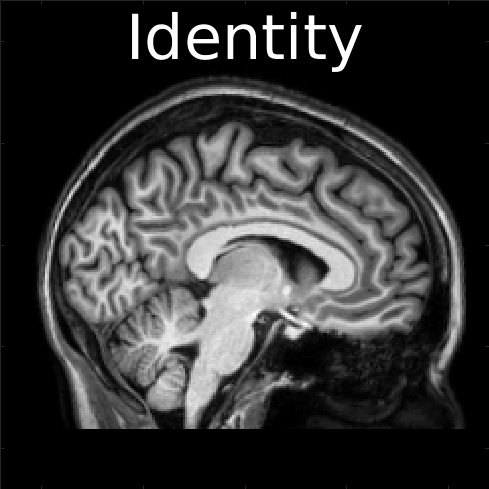
\includegraphics[width=0.15\textwidth]{ex2_id}
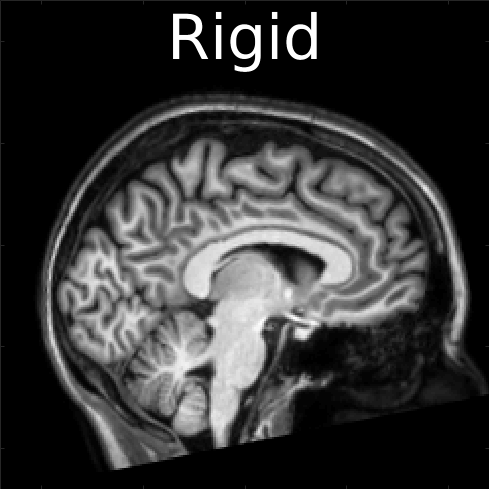
\includegraphics[width=0.15\textwidth]{ex2_rigid}
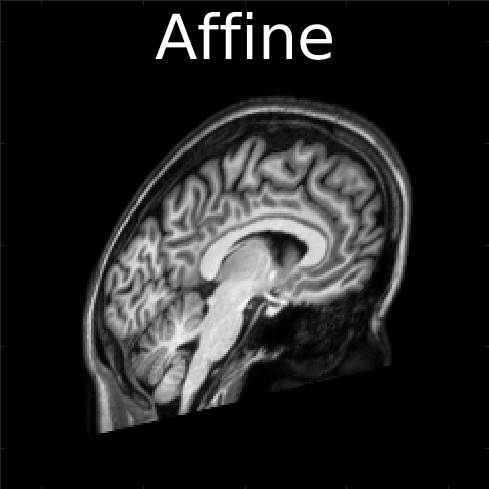
\includegraphics[width=0.15\textwidth]{ex2_affine}
%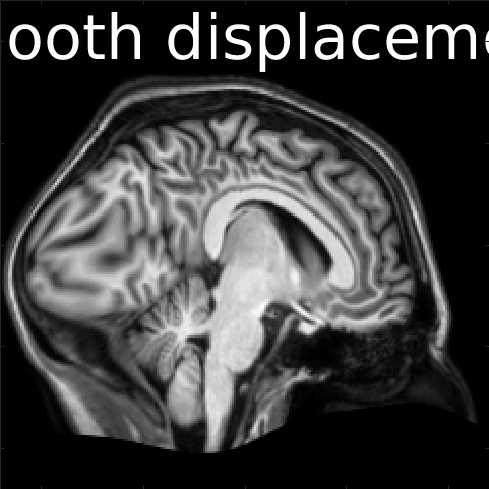
\includegraphics[width=0.2\textwidth]{ex2_disp}
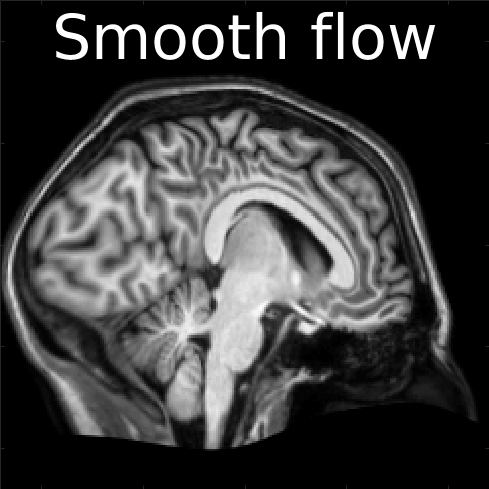
\includegraphics[width=0.15\textwidth]{ex2_flow}



\vspace{1em}
Regularization: How likely is a given transformation?

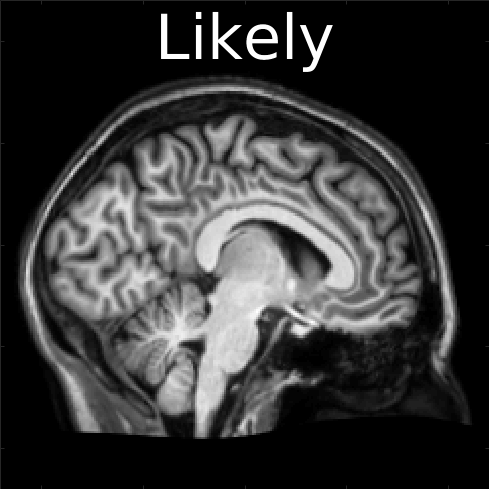
\includegraphics[width=0.15\textwidth]{ex2_flow_n_1}
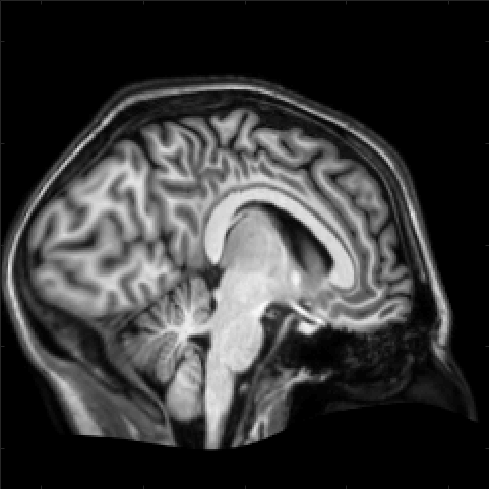
\includegraphics[width=0.15\textwidth]{ex2_flow_n_2}
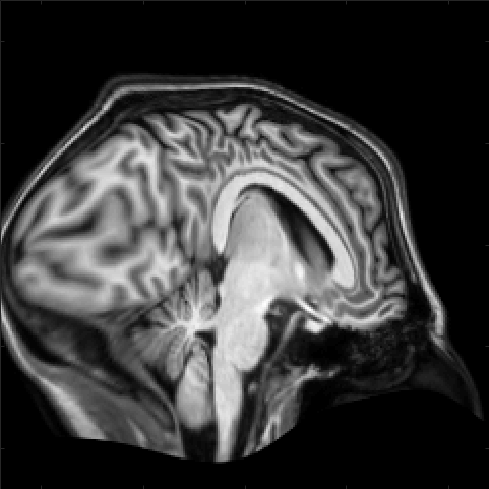
\includegraphics[width=0.15\textwidth]{ex2_flow_n_3}
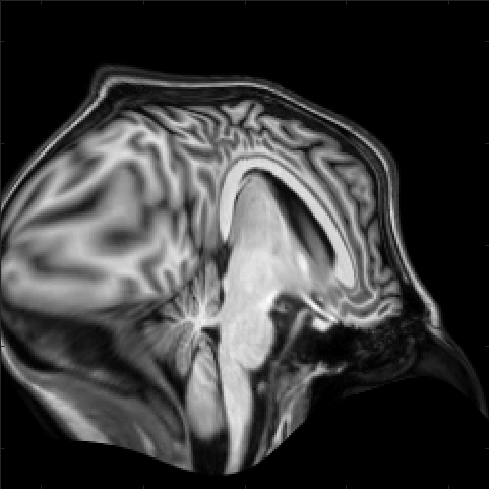
\includegraphics[width=0.15\textwidth]{ex2_flow_n_4}
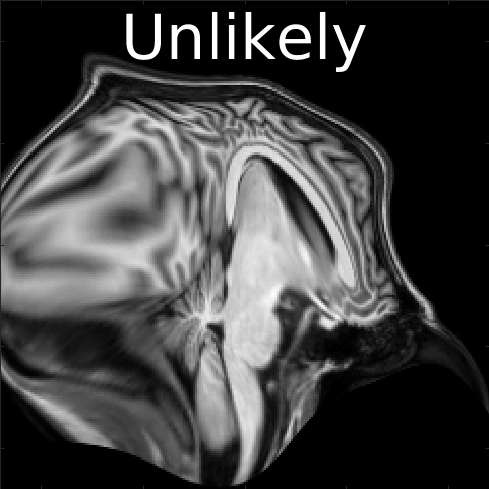
\includegraphics[width=0.15\textwidth]{ex2_flow_n_5}



\vspace{1em}
Similarity: How good is an alignment?

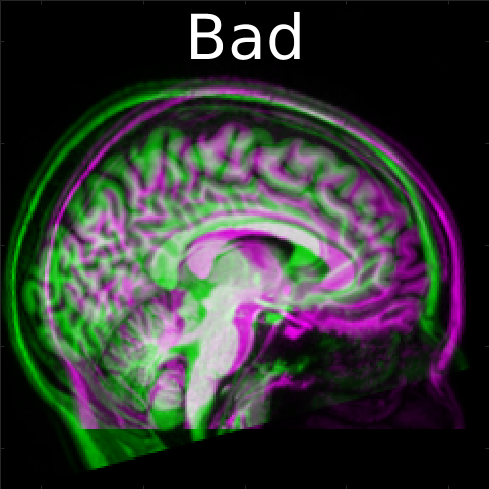
\includegraphics[width=0.15\textwidth]{ex2_affine_n_1}
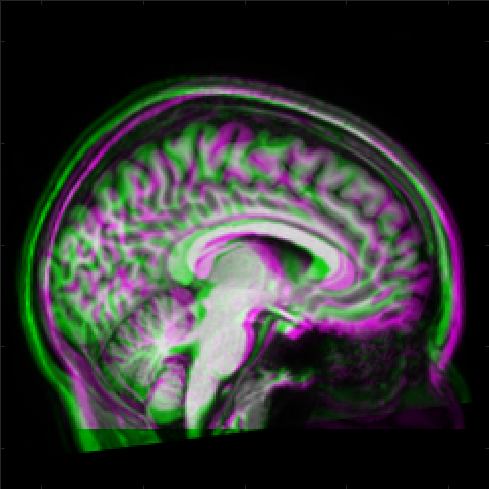
\includegraphics[width=0.15\textwidth]{ex2_affine_n_2}
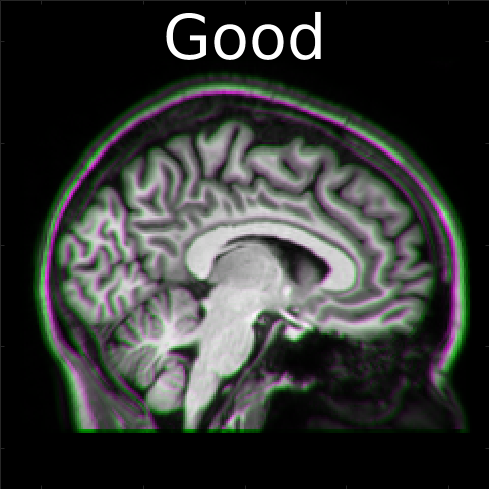
\includegraphics[width=0.15\textwidth]{ex2_affine_n_3}
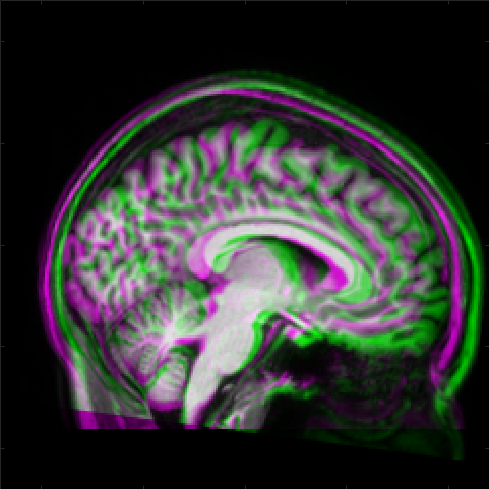
\includegraphics[width=0.15\textwidth]{ex2_affine_n_4}
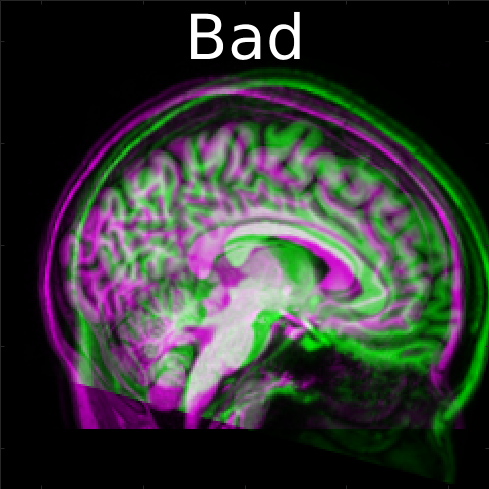
\includegraphics[width=0.15\textwidth]{ex2_affine_n_5}


\end{frame}


% extra frame for workshop
\begin{frame}{Transformation models: Matrix groups}

Euclidean (6 degrees of freedom): Encodes position and pose

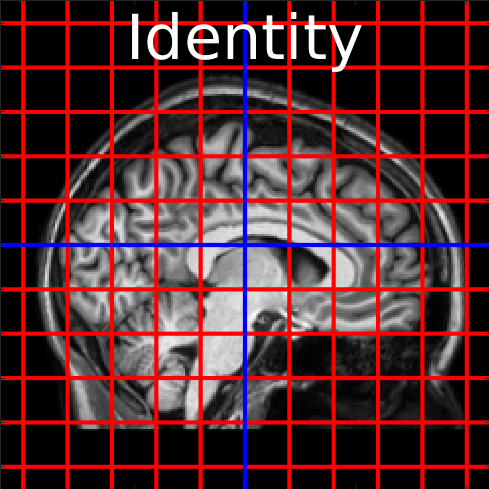
\includegraphics[width=0.15\textwidth]{tform_models_id}~
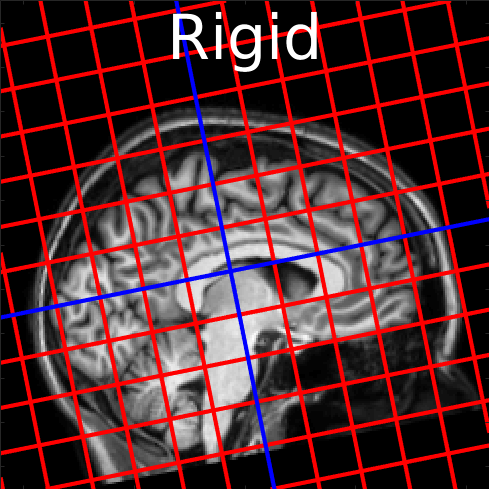
\includegraphics[width=0.15\textwidth]{tform_models_rigid_1}~
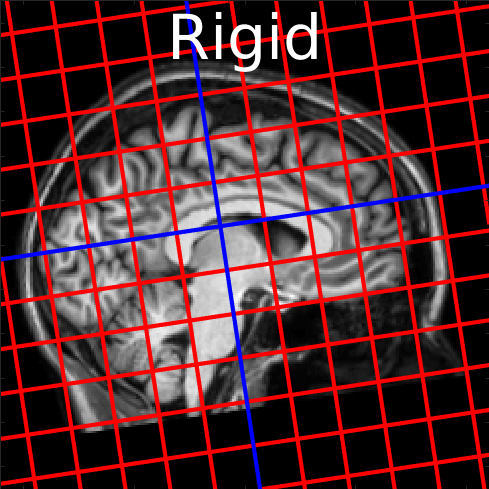
\includegraphics[width=0.15\textwidth]{tform_models_rigid_2}~
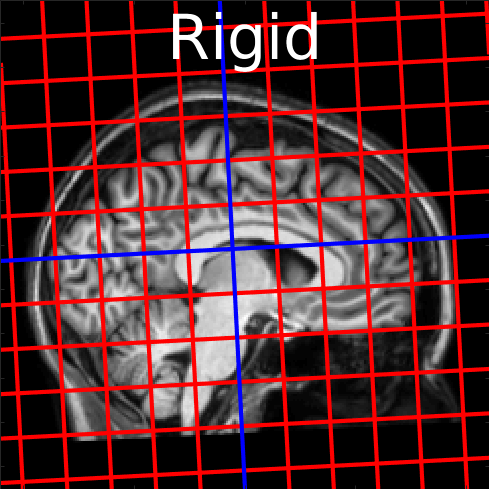
\includegraphics[width=0.15\textwidth]{tform_models_rigid_3}~
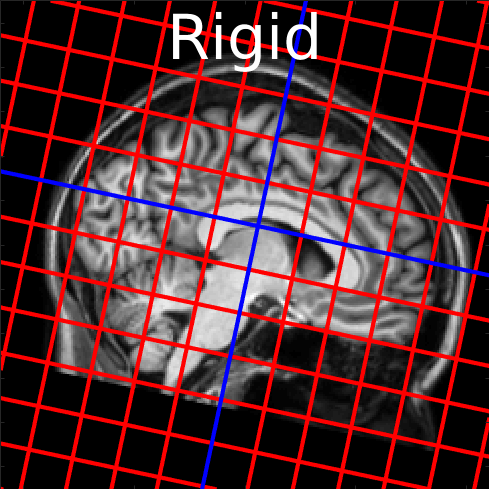
\includegraphics[width=0.15\textwidth]{tform_models_rigid_4}~
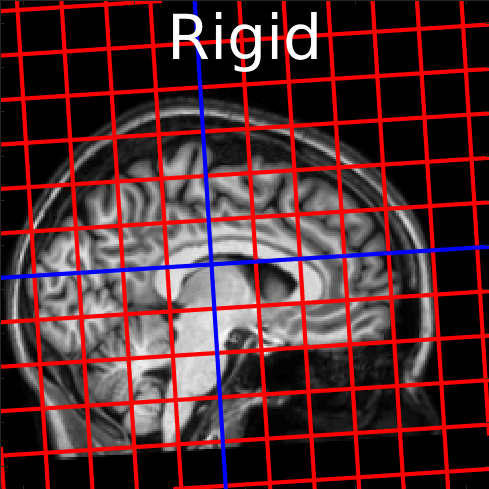
\includegraphics[width=0.15\textwidth]{tform_models_rigid_5}




Similarity (7 DOF): Include scale, more flexible, no shape change


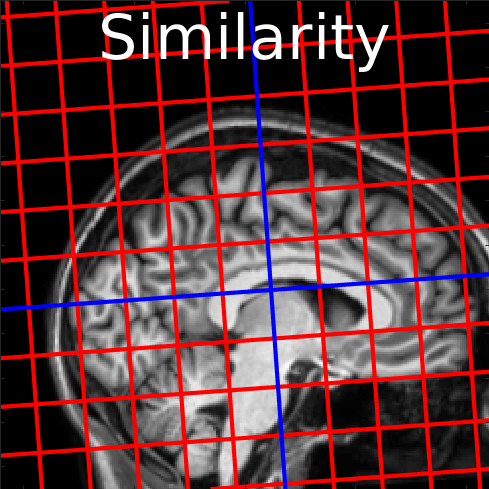
\includegraphics[width=0.15\textwidth]{tform_models_similarity_1}~
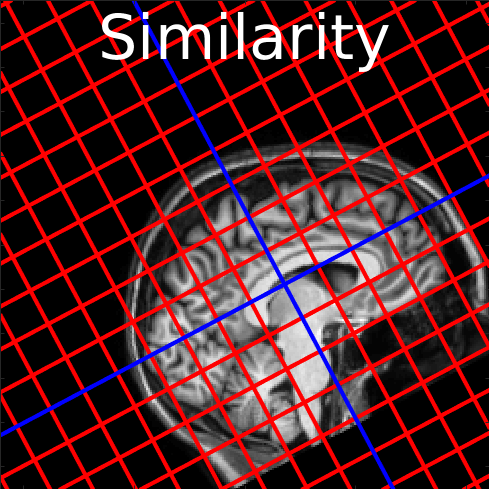
\includegraphics[width=0.15\textwidth]{tform_models_similarity_2}~
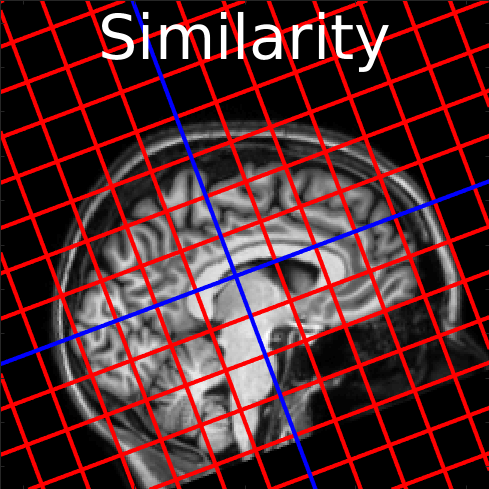
\includegraphics[width=0.15\textwidth]{tform_models_similarity_3}~
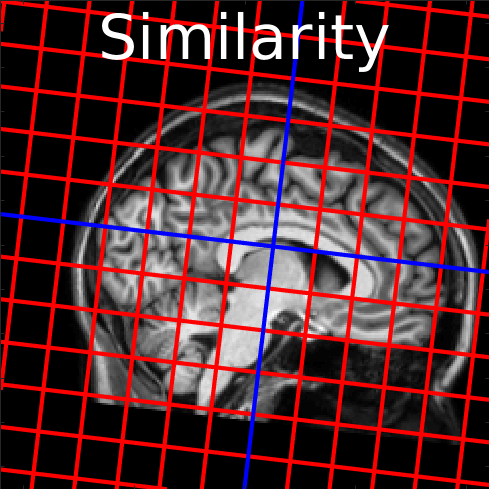
\includegraphics[width=0.15\textwidth]{tform_models_similarity_4}~
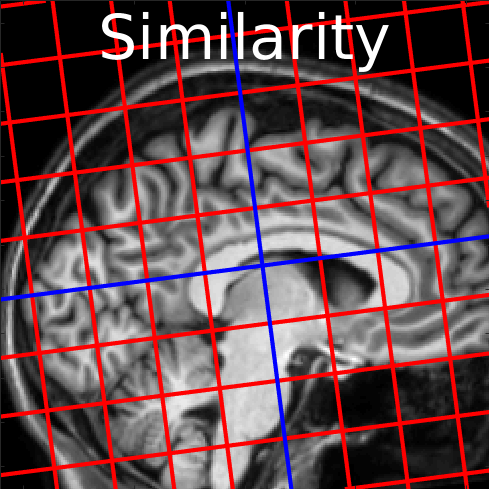
\includegraphics[width=0.15\textwidth]{tform_models_similarity_5}~
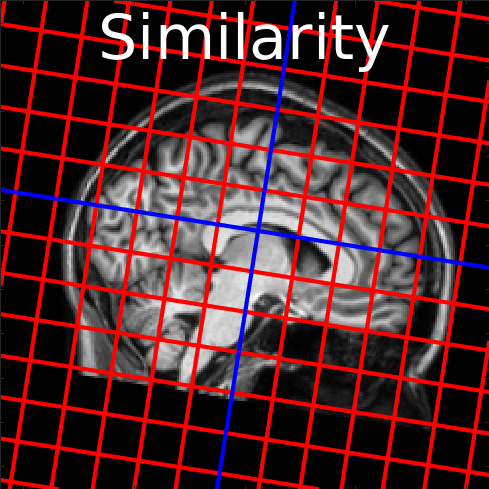
\includegraphics[width=0.15\textwidth]{tform_models_similarity_6}


Affine (12 parameters): Include shear and nonuniform scale


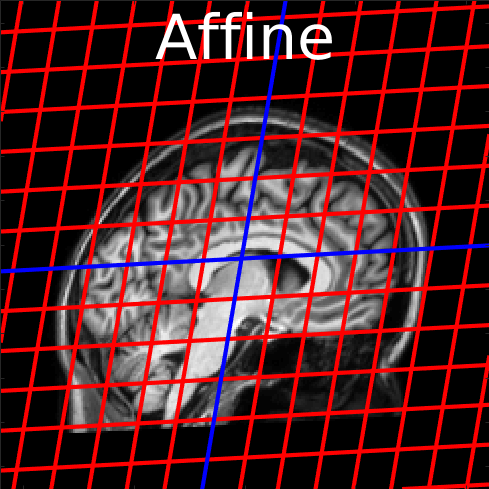
\includegraphics[width=0.15\textwidth]{tform_models_affine_1}~
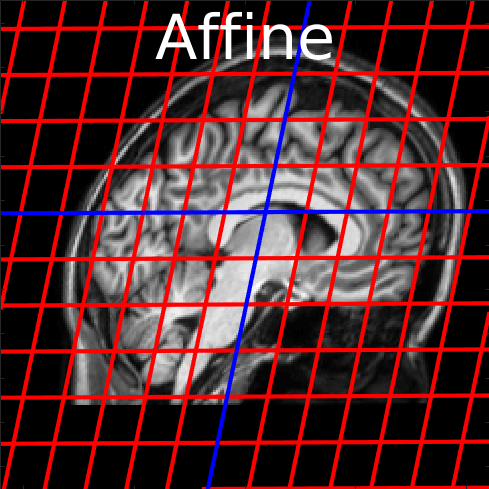
\includegraphics[width=0.15\textwidth]{tform_models_affine_2}~
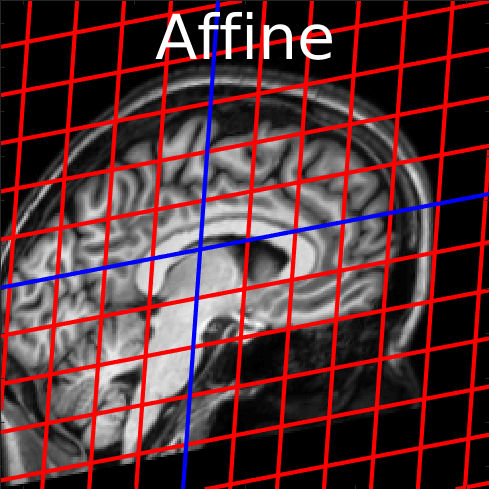
\includegraphics[width=0.15\textwidth]{tform_models_affine_3}~
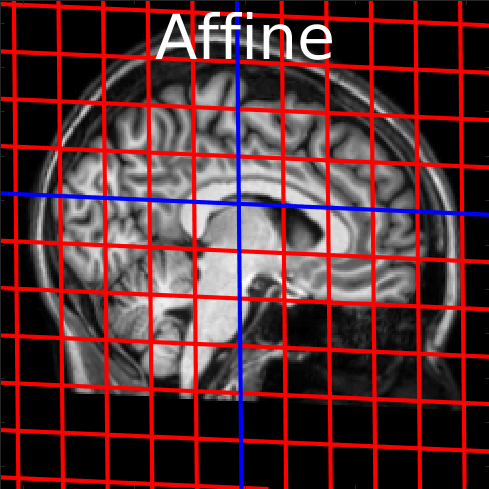
\includegraphics[width=0.15\textwidth]{tform_models_affine_4}~
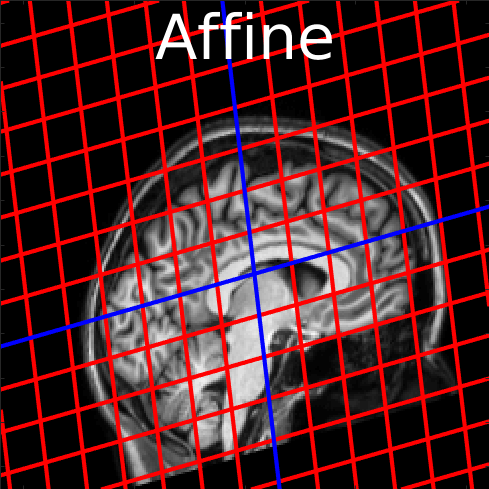
\includegraphics[width=0.15\textwidth]{tform_models_affine_5}~
\includegraphics[width=0.15\textwidth]{tform_models_affine_6}

\alert{Pros}: Simple to compute, easy to enforce invertibility, good for within-subject, often used in conjunction with deformations

\alert{Cons}: Cannot model distortions or realistic biological variability


\end{frame}

\begin{frame}{Transformation models: Displacement fields}


Can vary in magnitude
\includegraphics[width=0.15\textwidth]{tform_models_disp_4_1}~
\includegraphics[width=0.15\textwidth]{tform_models_disp_4_2}~
\includegraphics[width=0.15\textwidth]{tform_models_disp_4_3}~
\includegraphics[width=0.15\textwidth]{tform_models_disp_4_4}~
\includegraphics[width=0.15\textwidth]{tform_models_disp_4_5}~
\includegraphics[width=0.15\textwidth]{tform_models_disp_4_6}



or in smoothness
\includegraphics[width=0.15\textwidth]{tform_models_disp_1_4}~
\includegraphics[width=0.15\textwidth]{tform_models_disp_2_4}~
\includegraphics[width=0.15\textwidth]{tform_models_disp_3_4}~
\includegraphics[width=0.15\textwidth]{tform_models_disp_4_4}~
\includegraphics[width=0.15\textwidth]{tform_models_disp_5_4}~
\includegraphics[width=0.15\textwidth]{tform_models_disp_6_4}


\alert{Pros}: Can model a wide range of biological variability.

\alert{Cons}:  Large transforms fail to be invertible no matter how smooth

\includegraphics[width=0.15\textwidth]{tform_models_disp_1}~
\includegraphics[width=0.15\textwidth]{tform_models_disp_2}~
\includegraphics[width=0.15\textwidth]{tform_models_disp_3}~
\includegraphics[width=0.15\textwidth]{tform_models_disp_4}~
\includegraphics[width=0.15\textwidth]{tform_models_disp_5}~
\includegraphics[width=0.15\textwidth]{tform_models_disp_6}

\end{frame}

\begin{frame}{Transformation models: Flow fields}

Composition of invertible transforms is invertible. 

We use this to move from displacement to velocity.  

If $\Delta t v_i$ is a small displacement field, then the composition

$$\varphi_n = (id + \Delta t v_n)\circ \cdots \circ (id + \Delta t v_2) \circ (id + \Delta t v_1)$$
becomes a flow
$$
\frac{1}{\Delta t} (\varphi_{n+1} - \varphi_n) = v_n( \varphi_n ) \to \frac{d}{dt}\varphi_t = v_t(\varphi_t) 
$$
which gives Euler's equation in the limit.


\includegraphics[width=0.15\textwidth]{tform_models_flow_1}~
\includegraphics[width=0.15\textwidth]{tform_models_flow_2}~
\includegraphics[width=0.15\textwidth]{tform_models_flow_3}~
\includegraphics[width=0.15\textwidth]{tform_models_flow_4}~
\includegraphics[width=0.15\textwidth]{tform_models_flow_5}~
\includegraphics[width=0.15\textwidth]{tform_models_flow_6}

These \alert{diffeomorphisms} form the basis of \alert{Computational Anatomy}, as well as state of the art image registration algorithms.

\alert{Pros}: Geometric and statistical advantages (discussed below).

\alert{Cons}: Computational complexity.

\end{frame}



% extra for workshop
\begin{frame}{Regularization}

High dimensional transformations are not unique, regularization allows us to choose \alert{most favorable}.

\vspace{1em}

Early approaches used (e.g.) elastic energy.  For $\varphi$ a transform:

$$\int \frac12 |D(\varphi-id)(x)|^2_F dx$$

\vspace{1em}

Computational Anatomy\footnote{Beg, M. Faisal, et al. "Computing large deformation metric mappings via geodesic flows of diffeomorphisms." International journal of computer vision 61.2 (2005): 139-157.} uses kinetic energy Lagrangian:
\begin{align*}
\int_0^1 \frac{1}{2} \int |Lv_t(x)|^2 dx dt
\end{align*}
where $L$ is an inertial (differential) operator.

\vspace{1em}

Choosing $L$ with sufficient derivatives \alert{guarantees} diffeomorphisms.



\end{frame}




\begin{frame}{Regularization}
\begin{center}
\only<1>{\includegraphics[width=0.9\textwidth]{{flow/LDDMM1}.png}}%
\only<2>{\includegraphics[width=0.9\textwidth]{{flow/LDDMM2}.png}}%
\only<3>{\includegraphics[width=0.9\textwidth]{{flow/LDDMM3}.png}}%
\only<4>{\includegraphics[width=0.9\textwidth]{{flow/LDDMM4}.png}}%
\only<5>{\includegraphics[width=0.9\textwidth]{{flow/LDDMM5}.png}}%
\only<6>{\includegraphics[width=0.9\textwidth]{{flow/LDDMM6}.png}}%
\only<7>{\includegraphics[width=0.9\textwidth]{{flow/LDDMM7}.png}}%
\only<8>{\includegraphics[width=0.9\textwidth]{{flow/LDDMM8}.png}}%
\only<9>{\includegraphics[width=0.9\textwidth]{{flow/LDDMM9}.png}}%
\only<10>{\includegraphics[width=0.9\textwidth]{{flow/LDDMM10}.png}}%
\only<11>{\includegraphics[width=0.9\textwidth]{{flow/LDDMM11}.png}}%
\only<12>{\includegraphics[width=0.9\textwidth]{{flow/LDDMM12}.png}}%
\only<13>{\includegraphics[width=0.9\textwidth]{{flow/LDDMM13}.png}}%
\end{center}
\vspace{-1em}
Puts shapes and diffeomorphisms in a Reimannian \alert{metric space}.

\vspace{0.05em }

Allows statistical concepts such as averages or regression.

\end{frame}


\begin{frame}{Regularization}

Energy minimizing flows admit sparse solutions, key for overcoming bias variance tradeoff in high dimensions%, and multiple comparisons in statistics

\vspace{0.25em}
Regularization based on low dimensional priors for MAP estimates\footnote{Tward, Daniel, et al. "Parametric surface diffeomorphometry for low dimensional embeddings of dense segmentations and imagery." IEEE transactions on pattern analysis and machine intelligence (2016).}
\vspace{-1.5em}
\begin{center}
\includegraphics[width=0.8\textwidth]{Array.png}%
\end{center}
\end{frame}





% extra for workshop
\begin{frame}{Similarity: Feature point based}

Matching corresponding pairs of fiducial landmark points, {\color{cyan}$X$} to {\color{red}$Y$}, via sum of square error admits closed form solutions:
\begin{align*}
&\left.
\begin{array}{l}
\varphi(x) = Ax\\
 A = \text{Cov}(X,X)^{-1}\text{Cov}(X,Y)
\end{array}
\right\} \qquad  \text{(affine)}\\
&\left. 
\begin{array}{l}
\varphi(x) = x + \sum_i K(x,X_i) P_i\\
P = K(X,X)^{-1}(Y-X)
\end{array}
\right \} \qquad  \text{(spline displacement)}
\end{align*}
%Picture? Check course talks
\begin{center}
\includegraphics[width=0.28\textwidth]{landmarks0}
\includegraphics[width=0.28\textwidth]{landmarks2}
\includegraphics[width=0.28\textwidth]{landmarks3}
\end{center}
\vspace{-1.5em}
\vspace{1em}

Unlabeled points curves and surfaces via currents or varifolds.

\vspace{1em}
Points require manual selection, only ensures accuracy nearby.



\end{frame}



\begin{frame}{Similarity: Image based}
Common cost functions for comparing atlas $I(\varphi^{-1})$ to target $J$:

\vspace{1em}


\alert{Voxel based (intra modality)}, e.g. sum of square error
$$
\int \frac12 |I(\varphi^{-1}(x)) - J(x)|^2 dx
$$
conditional \alert{likelihood} of $J$ given $\varphi$ in a Gaussian white noise model.  

Other robust similarities can be used such as L1 or Huber.

\vspace{1em}


\alert{Neighborhood based (inter modality)}, e.g. MIND\footnote{Heinrich, Mattias P., et al. ``MIND: Modality independent neighbourhood descriptor for multi-modal deformable registration.'' Medical image analysis 16.7 (2012): 1423-1435.} or other local structure, local cross correlation.

\vspace{1em}

\alert{Histogram based  (inter modality)}, e.g. mutual information.



\end{frame}








\begin{frame}{Challenges and solutions}

Most brain mapping techniques were developed for medical imaging, but  neuroscience data faces unique challenges:


\begin{itemize}


\item 
Incomplete or sliced data

\item 
Artifacts or damaged tissue

\item 
Multiple different modalities or appearance

\end{itemize}

\includegraphics[width=\textwidth,clip,trim=0in 1.3in 0in 0in]{720exampleslices-edit}

\vspace{1em}

We use machine learning to predict one image from another, while \alert{jointly} performing registration and artifact detection\footnote{ Tward, Daniel Jacob, et al. ``Diffeomorphic registration with intensity transformation and missing data: Application to 3D digital pathology of Alzheimer's disease.'' BioRxiv (2019): 494005.}

\vspace{1em}
\includegraphics[width=\textwidth,clip,trim=0in 0in 0in 1.3in]{720exampleslices-edit}


\end{frame}

% extra for workshop
\begin{frame}{Intensity mapping: \only<1>{Grayscale to grayscale}\only<2>{Grayscale to RGB}\only<3>{RGB to RGB}}
%\blfootnote{Tward, Daniel Jacob, et al. ``Diffeomorphic registration with intensity transformation and missing data: Application to 3D digital pathology of Alzheimer's disease.'' BioRxiv (2019): 494005.}

Expand optimization problem to include an intensity transform $F_\theta$
\begin{align*}
\int \frac12 |\alert{F_\theta} [I(\varphi^{-1}(x))] - J(x)|^2 dx
\end{align*}
and optimize jointly over $\varphi$  and $\theta$.
\only<1>{
\vspace{-0.5em}
\begin{center}
\includegraphics[height=0.64\textheight]{intensity_example_1.png}
\end{center}
\vspace{-0.5em}
Calibration curve: reduce contrast at low intensity, increase at high.
}%
\only<2>{
\vspace{-0.5em}
\begin{center}
\includegraphics[height=0.64\textheight]{intensity_example_2.png}
\end{center}
\vspace{-0.5em}
Nonmonotonic: swaps order of ``grey'', ``white'', ``background''.
}%
\only<3>{
\vspace{-0.5em}
\begin{center}
\includegraphics[height=0.64\textheight]{intensity_example_3.png}
\end{center}
\vspace{-0.5em}
Mix powers of RGB, fairly high dimensional, flexible transforms.  
}%

\end{frame}








% extra for workshop
\begin{frame}{Artifacts}
%\blfootnote{Tward, Daniel Jacob, et al. ``Diffeomorphic registration with intensity transformation and missing data: Application to 3D digital pathology of Alzheimer's disease.'' BioRxiv (2019): 494005.}

Allows multimodality registration with simple Gaussian likelihood.


Handle artifacts with Expectation Maximization algorithm
\begin{align*}
\int \frac12 |\alert{F_\theta} [I(\varphi^{-1}(x))] - J(x)|^2\alert{W(x)} dx
\end{align*}

\alert{E step}: Compute $W$ as posterior probability for fixed $\theta,\varphi$.

\alert{M step}: Compute optimal $\theta,\varphi$ for fixed $W$.


%In this simulated example we find tissue labels, estimate nonmonotonic intensity transformation, and diffeomorphism (left).

%Existing approaches (right) fail on this simple example.

\centering
\fbox{
\includegraphics[width=0.68\textwidth,clip,trim=0.5in 0in 0in 0in]{phantom_1.png}
}~
\fbox{
\includegraphics[width=0.24\textwidth,clip,trim=0.5in 0in 10.9in 0in]{phantom_2.png}
}
\end{frame}


\begin{frame}{Multimodality and damaged tissue in digital pathology}
\phantom{.}\hfill
\includegraphics[height=0.9\textheight]{missing_data_different_intensity_digital_pathology.png}
\hfill\phantom{.}
\end{frame}

\begin{frame}{Multimodal 2D histology slices to 3D atlas}

\phantom{.}\hfill
\includegraphics[width=0.9\textwidth]{all_slices.png}
\hfill\phantom{.}

\end{frame}

\begin{frame}{CLARITY cleared mouse brain registered to Allen Atlas}

\includegraphics[width=\textwidth]{CLARITY_mouse_registration.png}

\end{frame}




\begin{frame}{ARDENT\footnote{Affine and Regularized Diffeomorphic Numeric Transform.  $^8$Tward, Daniel, et al. ``Parametric surface diffeomorphometry for low dimensional embeddings of dense segmentations and imagery. IEEE transactions on pattern analysis and machine intelligence (2016) $^9$Tward, Daniel, et al. ``Estimating diffeomorphic mappings between templates and noisy data: Variance bounds on the estimated canonical volume form. Quarterly of Applied Mathematics (2019). }: NeuroData's open source brain mapping tool }

Publications and code available online from \url{neurodata.io/reg}


%\begin{itemize}
%\item Transformation model: Diffeomorphism group allows flexible deformations guaranteed smooth and invertible
%\item Similarity: Negative log likelihood allows statistical approaches to missing data and multiple modalities
%\item Regularization: Flow kinetic energy enables sparse representations effective in high dimensional bias variance tradeoff.
%\end{itemize}

\vspace{-1.5em}

\begin{table}
\begin{tabular}{p{2.1cm}p{2.3cm}p{5.3cm}}
Ingredient & Choice & Benefit\\
\hline
\hline
Transform & Diffeomorphism & Smooth invertible fluid transform\\
\hline
Similarity & Log likelihood & Enables statistical approaches to artifacts and multi-modality\\
\hline
Regularization & Kinetic energy & Enables sparse representations effective in high dimensional bias variance tradeoff$^{5,6}$
\end{tabular}
\end{table}


\vspace{-1em}

\noindent
\begin{tikzpicture}
\tikzstyle{rect} = [rectangle,text width=2.5cm,text centered];
\node (atlas) [rect] at (-4.1cm,0cm) {\includegraphics[width=\textwidth,clip,trim=0.5in 0in 0.5in 0in]{ardent2}};
\node (bef) [rect] at (-1.6cm,0cm) {\includegraphics[width=\textwidth,clip,trim=0.5in 0in 0.5in 0in]{ardent0}};
\node (aft) [rect] at (1.6cm,0cm) {\includegraphics[width=\textwidth,clip,trim=0.5in 0in 0.5in 0in]{ardent1}};
\node (targ) [rect] at (4.1cm,0cm) {\includegraphics[width=\textwidth,clip,trim=0.5in 0in 0.5in 0in]{ardent3}};

\draw [->,thick] (bef) -- (aft);
\end{tikzpicture}

\end{frame}



% extra for workshop
\begin{frame}{Computation}%
\setcounter{footnote}{6}%
Computational burden\footnote{Tward, Daniel J., et al. "Performance of Image Matching in the Computational Anatomy Gateway: CPU and GPU Implementations in OpenCL." Proceedings of the Practice and Experience in Advanced Research Computing 2017 on Sustainability, Success and Impact. ACM, 2017.} includes interpolation:
\begin{itemize}
\item integrating flows
\item deforming images
\end{itemize}
and Fast Fourier Transforms:
\begin{itemize}
\item applying differential operators
\item inverting differential operators
\end{itemize}
both are very efficiently parallelized.

\vspace{1em}

We use pytorch (\url{pytorch.org}) as interface to GPU computing.

\vspace{1em}

Registration algorithm is about 200 lines of code.

\vspace{1em}

Optimization with gradient descent.

\end{frame}



\begin{frame}{Acknowledgements}

\begin{columns}
\begin{column}{0.5\textwidth}
People
\begin{itemize}
\item Michael Miller (JHU)
\item Joshua Vogelstein (JHU)
\item Susumu Mori (JHU)
\item Juan Troncoso (JHU)
\item Marilyn Albert (JHU)
\item Partha Mitra (CSHL)
\item Brian Lee (JHU)
\item Vikram Chandrashekhar (JHU)
\item Devin Crowley (JHU)

\end{itemize}
\end{column}

\begin{column}{0.5\textwidth}
Funding

\vspace{1em}

NIH: P41EB015909, R01NS086888, R01EB020062, R01NS102670, U19AG033655, R01MH105660, P50AG05146

\vspace{1em}

NSF: 16-569 NeuroNex contract 1707298, ACI1548562 (Extreme Science and Engineering Discovery Environment)

\vspace{1em}

Kavli Neuroscience Discovery Institute, BrightFocus Foundation, Dana Foundation

\end{column}
\end{columns}

\end{frame}





\end{document}